\section{Cisco}

  \subsection{Introduction}

  Cisco Systems is an industry leader who develops, manufactures and sells networking hardware, software, telecommunications equipment and other high-technology services and products.

  Cisco NX-OS nowadays is a  well-known network operating system in the market with a good amount of documentation, provider and partner support around the globe, and dedicated forums to access in order to seek knowledge alongside officials’ courses and certifications. Cisco NX-OS is also well known for being a data center-class operating system that includes the following feature and benefits:

  For features and benefits go to \href{https://www.cisco.com/c/en/us/products/collateral/ios-nx-os-software/nx-os-software/data_sheet_c78-652063.pdf}{Cisco-NXOS-DataSheet}

  The quotations made by Cisco partner, NTT Chile can be found on confluence under: \href{https://confluence.lsstcorp.org/display/IT/ITTN-043+-+Rubin+Network+Re-Engineering}{ITTN-043 Resources - Quotation}

\newpage

  \subsection{Hardware}

  Our actual data center network is based on Cisco hardware and ACI-oriented. The following image is a summary of summit and base actual ACI infrastructure:

\vspace{4 mm}

  \begin{figure}
    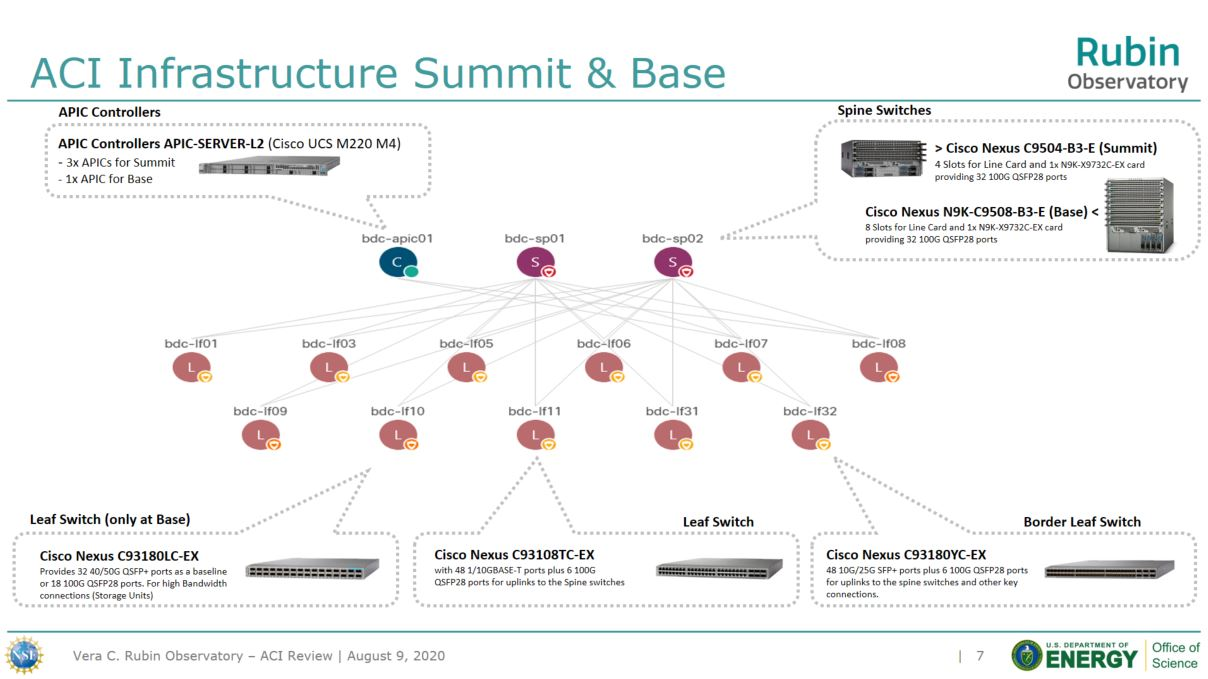
\includegraphics[width=15cm]{images/aci-infrastructure-summit-and-base.jpg}
    \centering
    \caption{Actual Summit and Base ACI Infrastructure}
  \end{figure}

  The leaves switches can be migrated into NXOS since the software cames from fabric, we require to migrate the spine switches to NXOS. For that we have two options:

  \begin{itemize}
    \item Option 1: Adquire NXOS software and licensing for spines switches, or
    \item Option 2: Adquire new spine switches for summit and base
  \end{itemize}

  The hardware required in any case will be the already in place which is:

  \begin{itemize}
    \item Summit: 2 units - Cisco Nexus C9504-B3-E - 4 Slots for Line Card and 1x N9K-X9732C-EX card providing 32 100G QSFP28 ports
    \item Base: 2 units - Cisco Nexus N9K-C9508-B3-E - 8 Slots for Line Card and 1x N9K-X9732C-EX card providing 32 100G QSFP28 ports
  \end{itemize}

\newpage


  \subsection{License}

  In order to go from ACI fabric to NX-OS, we were informed by Cisco and NTT that our leaves switches will require no further licensing since they came with NX-OS supported from fabric, but that was not the case for all the spine switches, who will require new licensing to support NX-OS when migrating from ACI operating system.

  Quotations were requested to Cisco/NTT for NX-OS Essentials software licenses for both spine switches models (C9504 and C9508). Quotes can be found here: \href{https://confluence.lsstcorp.org/display/IT/ITTN-043+-+Rubin+Network+Re-Engineering?preview=/151855733/156506276/quote_nxos_licenses_march2021.pdf}{NXOS-Essential-Licenses}

\newpage

  \subsection{Network Design}

  The network design is based on open-source protocols in order to avoid propietary protocols that could tied the network to an specific brand. The network design agreed by Rubin's IT Team is based first on NX-OS operating system, but using an MLAG aggregation core as spine switches, building a big layer 2 fabric at summit and base.

  The following topology explain on a high level design how the entire Rubin's network will look like:

  \begin{figure}
    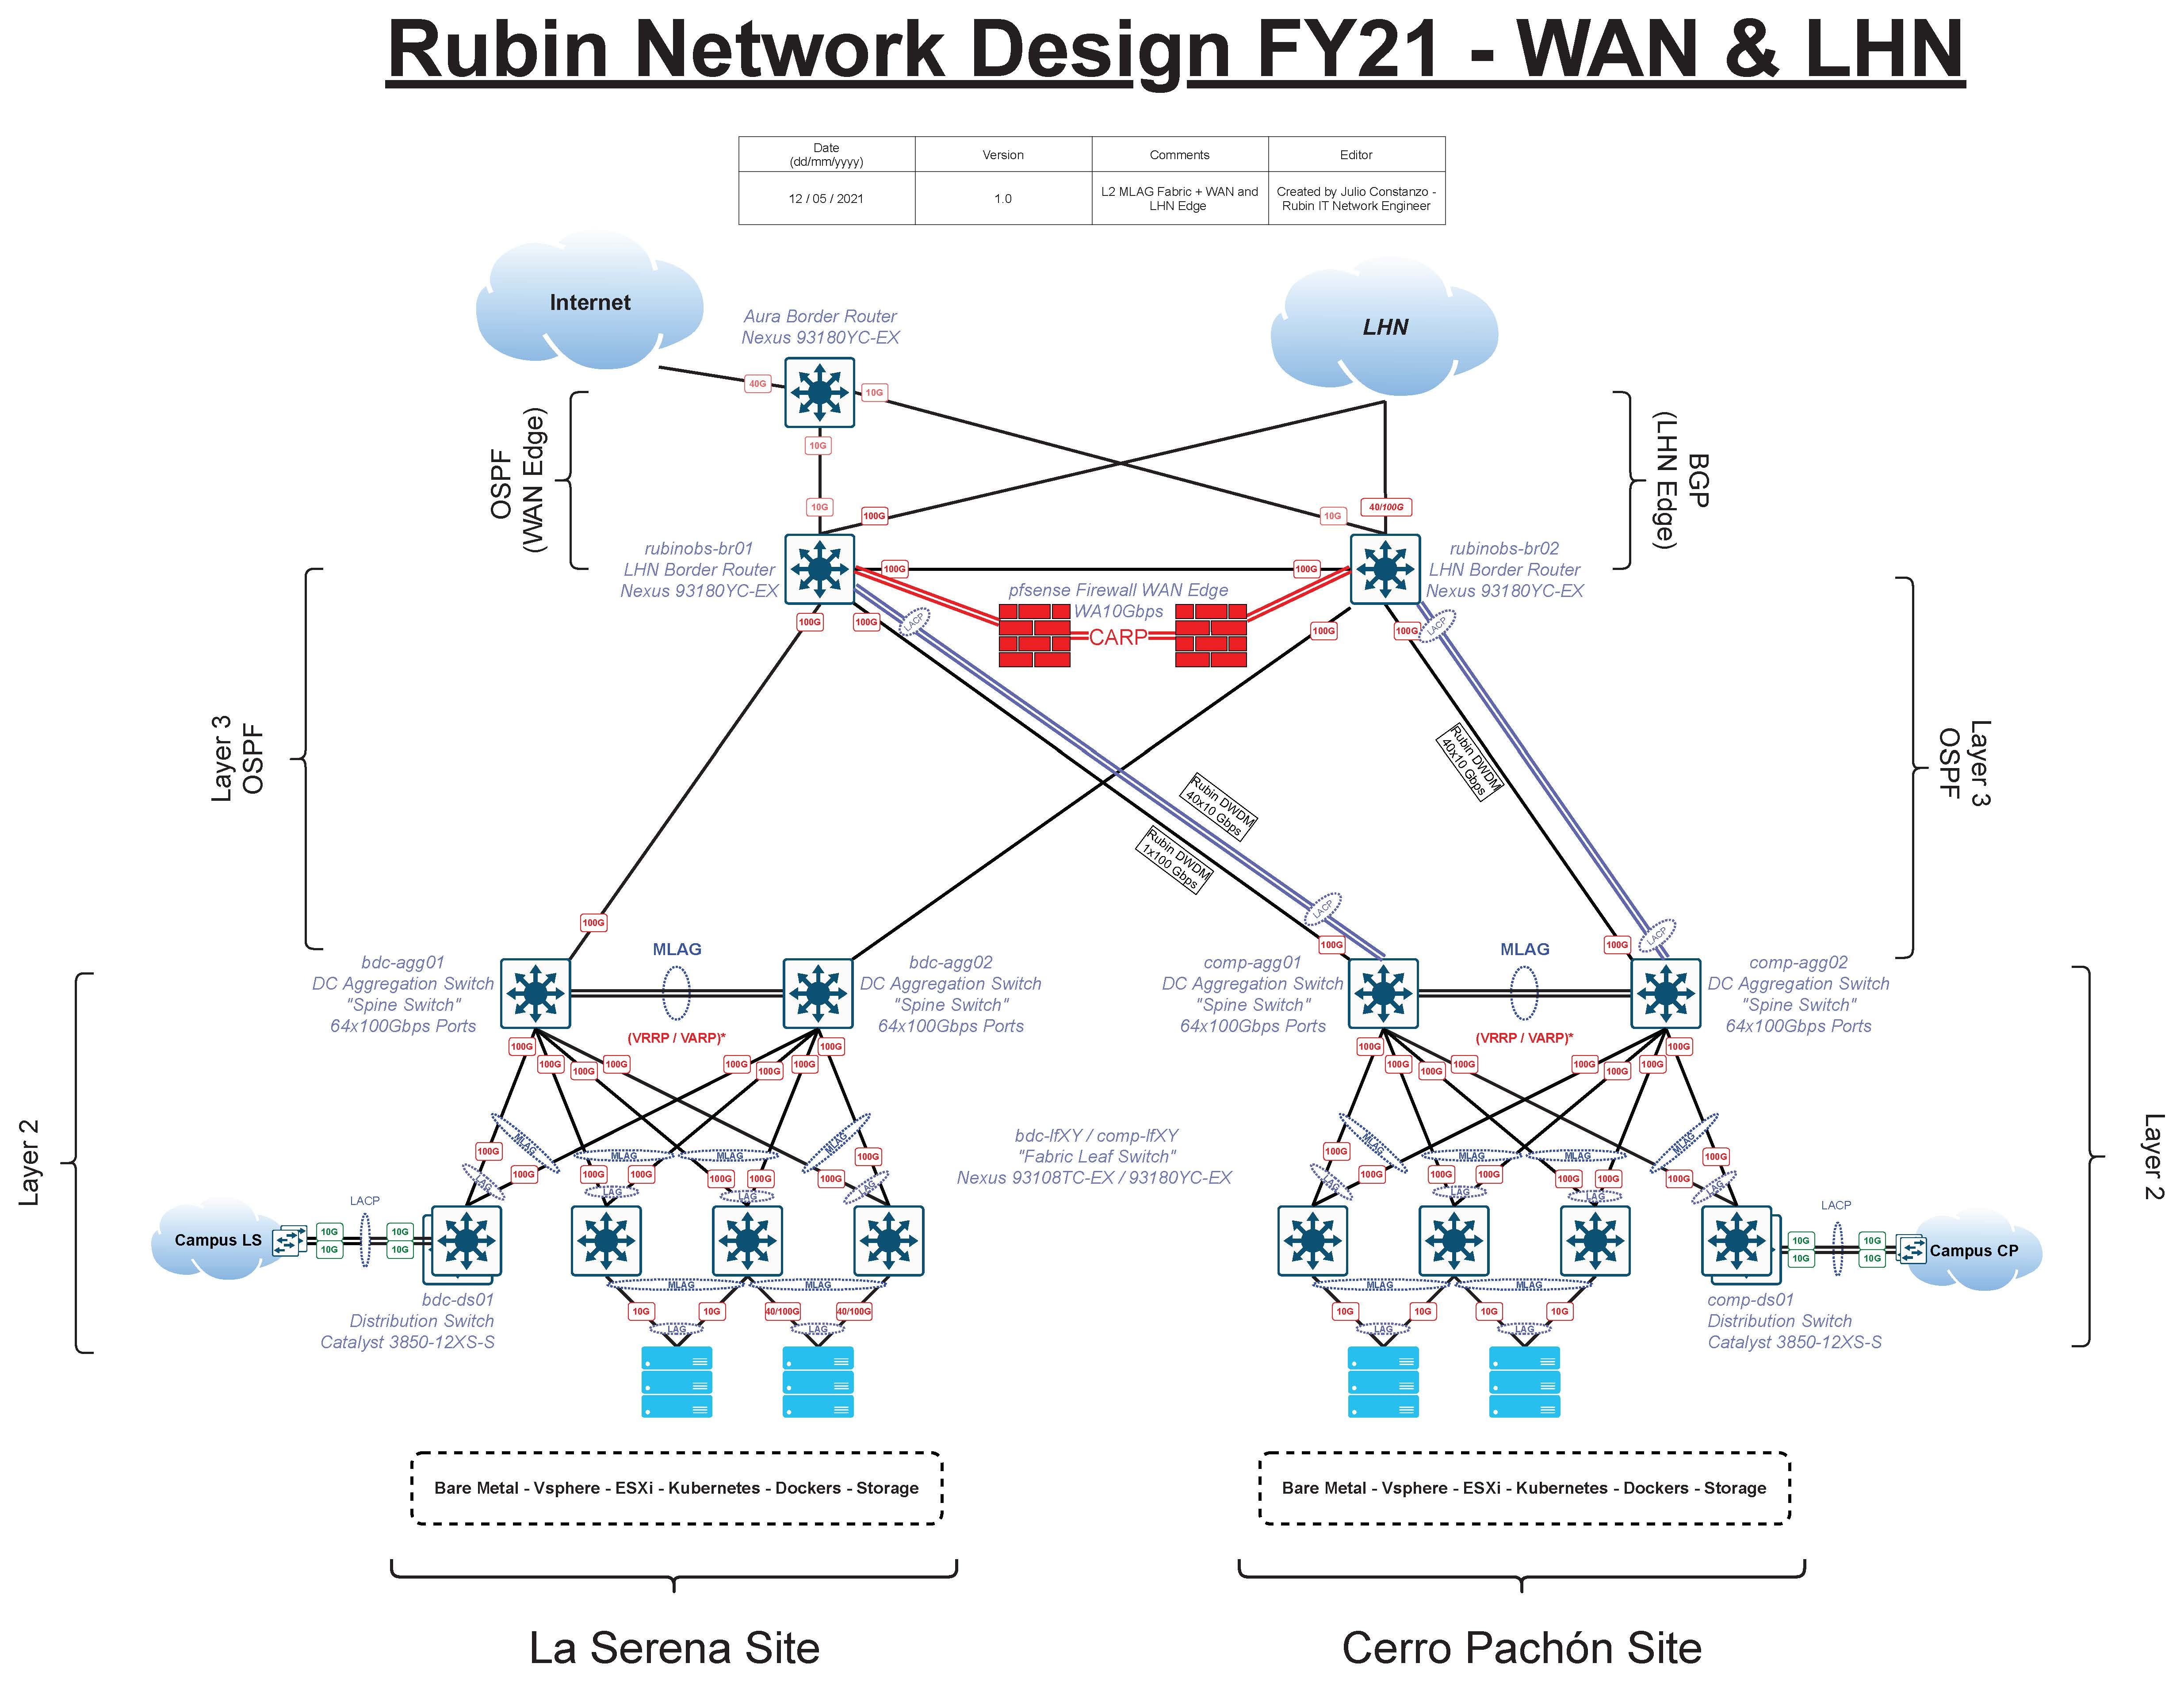
\includegraphics[width=15cm]{images/fy21-rubin-network.jpg}
    \centering
    \caption{FY21 Rubin Network Re-Design}
  \end{figure}

\newpage

  \subsection{Support}

  All quotation were requested and made with a 5-year support contract (8x5xNBD). Cisco also provides their specialist via Cisco TAC (Cisco Technical Assitance Center) which provides technical support to customers, partners and resellers.

  Cisco provides two types of support:

  \begin{itemize}
    \item Online at Cisco TAC website \href{http://www.cisco.com/tac}{Cisco TAC website}
    \item Via email/phone through the TAC Escalation Center
  \end{itemize}

  \subsection{Training}

  Cisco is well known for having a large amount of certifications paths in the market, which are also well valued by enterprises around the globe. Most of the training centres, if not all of them, have Cisco certifications paths into their training curses because of their market value and recognition. For more information about training and certifications please visit \href{https://www.cisco.com/c/en/us/training-events/training-certifications.html}{Cisco Training, Learning and Certifications} 




